

\section{datAcron Architecture}		
\frame
{		
	\frametitle{datAcron Architecture}
	\framesubtitle{}
	
	\begin{center}
		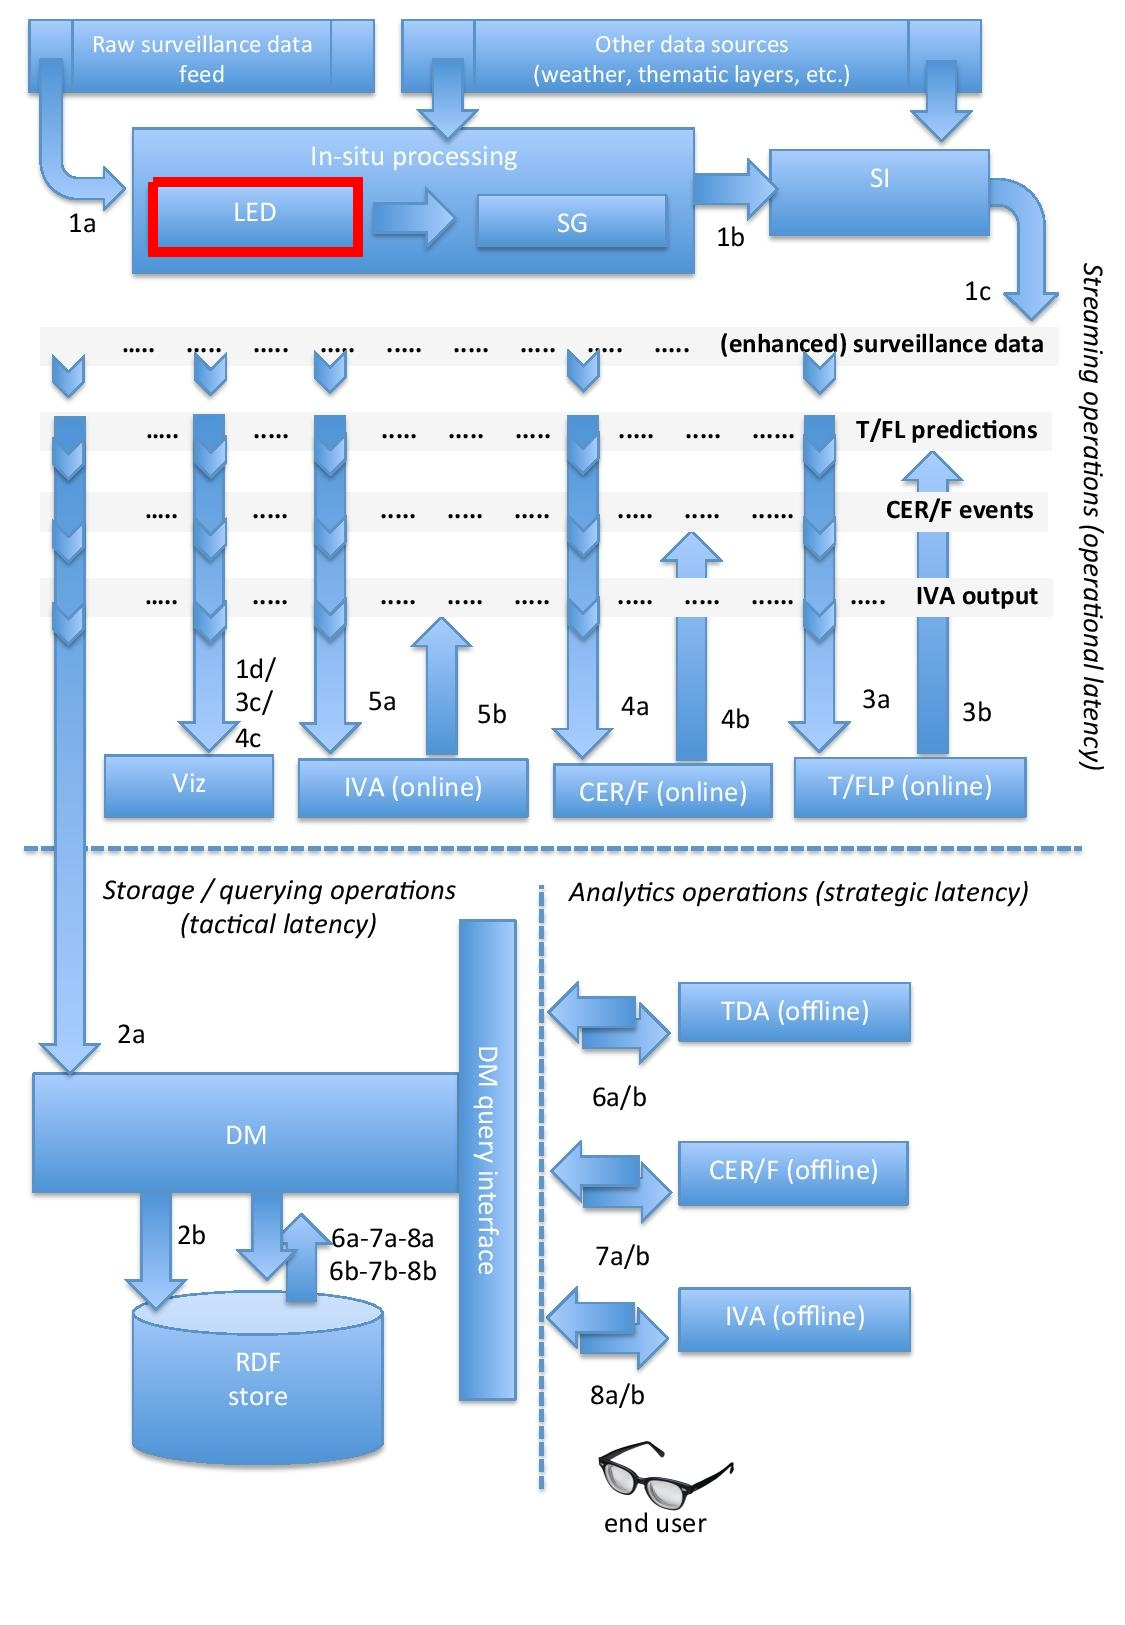
\includegraphics[width=.85\textwidth,height=.75\linewidth]{figures/arch1.jpg}\\
		.
	\end{center}
	
}

\section{Overview}
\frame
{
	\frametitle{In-situ (LED Component) \footnote{ github.com/ehabqadah/in-situ-processing-datAcron}}
	\framesubtitle{Overview}
		\begin{center}
			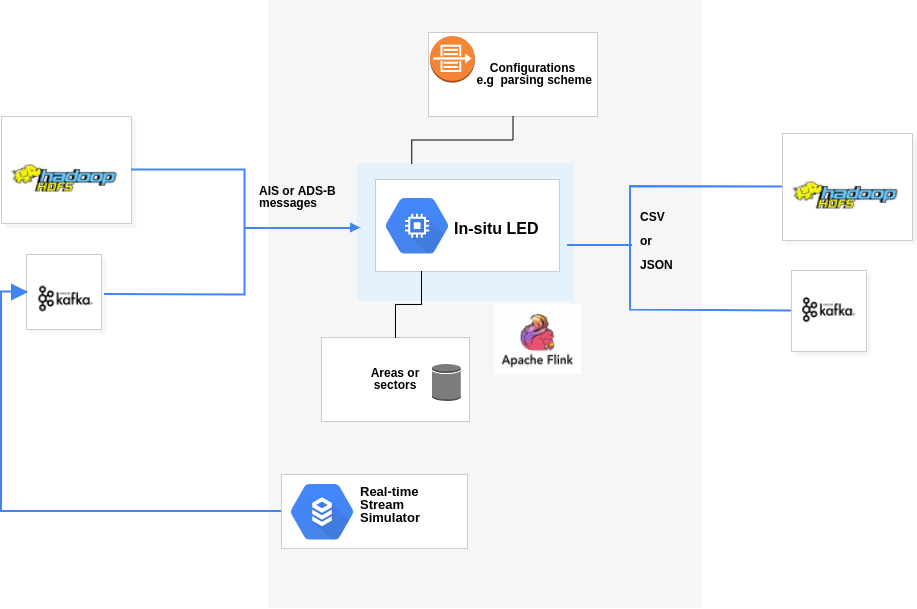
\includegraphics[scale=.32,left]{figures/insitu.png}\\
			.
		\end{center}
}


\frame
{
	\frametitle{In-situ LED}
	\framesubtitle{Functionalities}
	\begin{itemize}[]
	\item-Trajectory enrichment: computing trajectory statistics In-Situ
	\item	-e.g., min/max/mean/var speed, acceleration
	\item	-Deriving events against context information
    \item		-Monitoring of ADS-B messages against sector information
	\item	-Derivation of high-level events for sector entering and leaving
	\item	-High-level events will be provided as real-time stream for applications
		
	\end{itemize}
}

\frame
{
	\frametitle{Real-time stream simulator}
	
	\begin{itemize}[]
		\item<1->Given a set of $k$ real-time streams of events $S = \{ s_1,s_2, ..., s_k\}$.
		
		\item<1 -> Each stream $s_i=\langle e_1,e_3...,e_t,...\rangle$  is an evolving time-ordered sequence of events.
		
		\item<1 -> Each event is defined as a tuple of attributes $e_t = (type,\tau,id,a_1,a_2.....,a_n)$ where $type\ \in  \Sigma$ (i.e., event types). 
		\item<1-> A user-defined pattern (i.e., complex event of interest) $P$ expressed as sequence of event types.
		
		%  \item<1->Goal:  provides online prediction about when the event pattern $P$ is expected to be completed each single stream $s_i$ 
		
		\item<1->Goal: the main objective is to predict the pattern $P$ completion with certain probability in the future over each stream $s_i$ given the current time event $e_t$. 
	\end{itemize}
}


\section{Output Scheme}		
\frame
{		
\frametitle{Output CSV scheme (29 fields)}
\framesubtitle{}

\begin{center}
	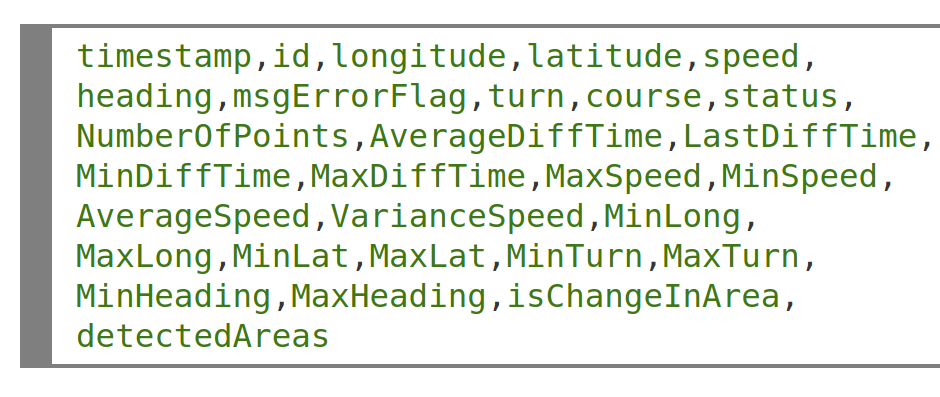
\includegraphics[scale=.32,left]{figures/insitu_output.png}\\
	.
\end{center}

}


\section{Deployment and Integration }
\frame
{	
	\frametitle{Deployment}
	\framesubtitle{}
migration from VM version to true cluster (including cluster details 10 nodes, 8 cores each)
}



\frame
{	
	\frametitle{In-situ deployment on datAcron YARN cluster}

	\begin{center}
		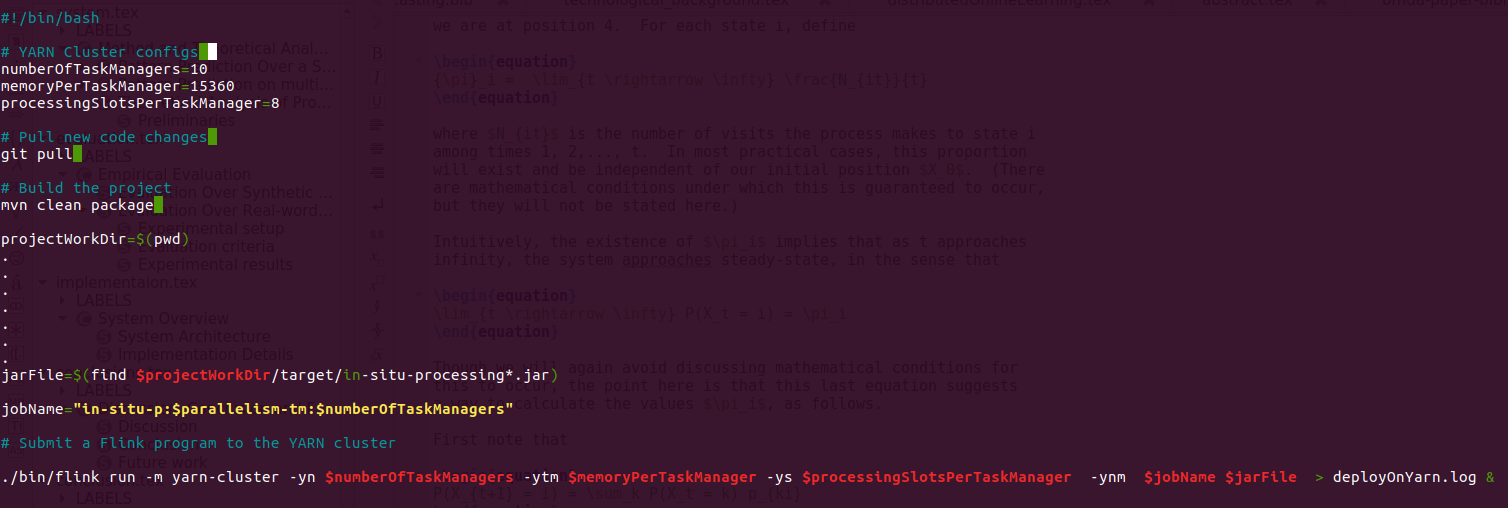
\includegraphics[width=.7\textwidth,height=.5\linewidth]{figures/deploy.png}
		.
	\end{center}
}


\section{Performance on YARN cluster}
\frame
{	
	\frametitle{In-situ Performance}
	\framesubtitle{Throughput on datAcron YARN cluster}
		\begin{center}
		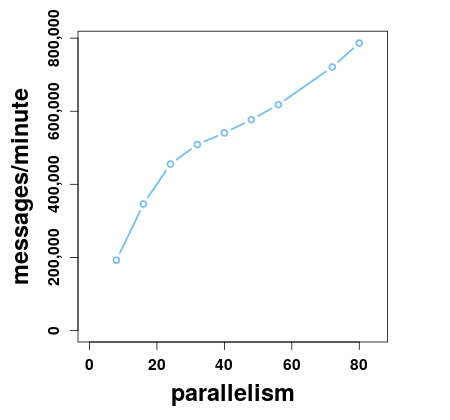
\includegraphics[width=.95\textwidth,height=.7\linewidth]{figures/throughput.png}
		.
	\end{center}
}


\section{Conclusion}
\frame
{	
	LED in-situ processing ressource/CPU consumption and delay
	can be neglected
}